\begin{figure}[t]
\centering
\subfigure[\gls{SLIC}]{%
  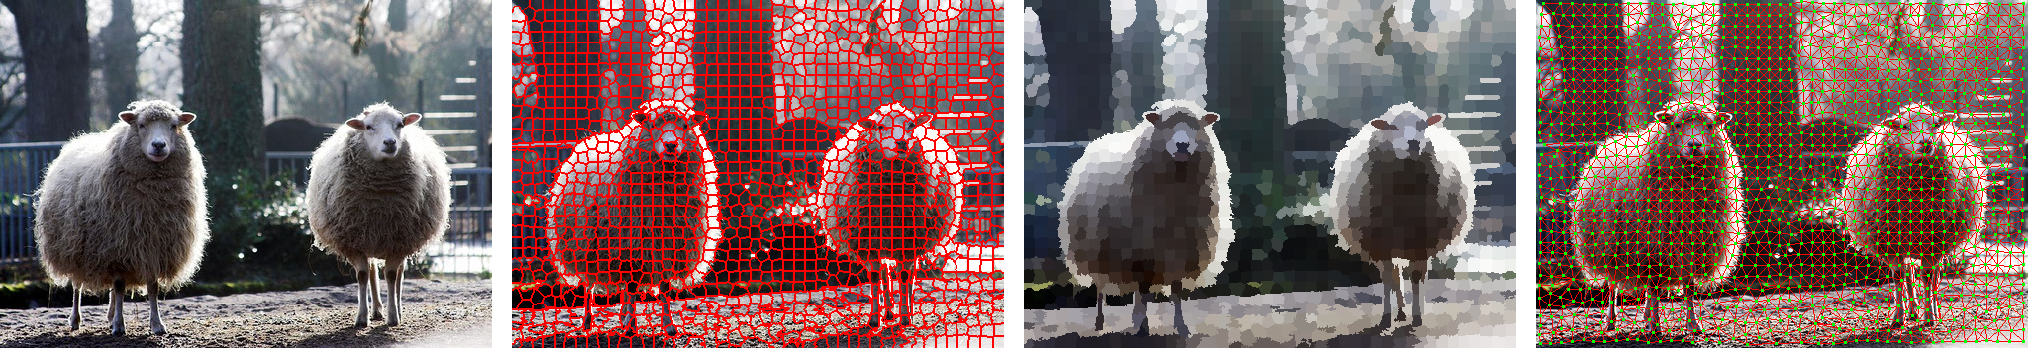
\includegraphics[width=\textwidth]{bilder/pascal_voc_slic.png}
}
\subfigure[Quickshift]{%
  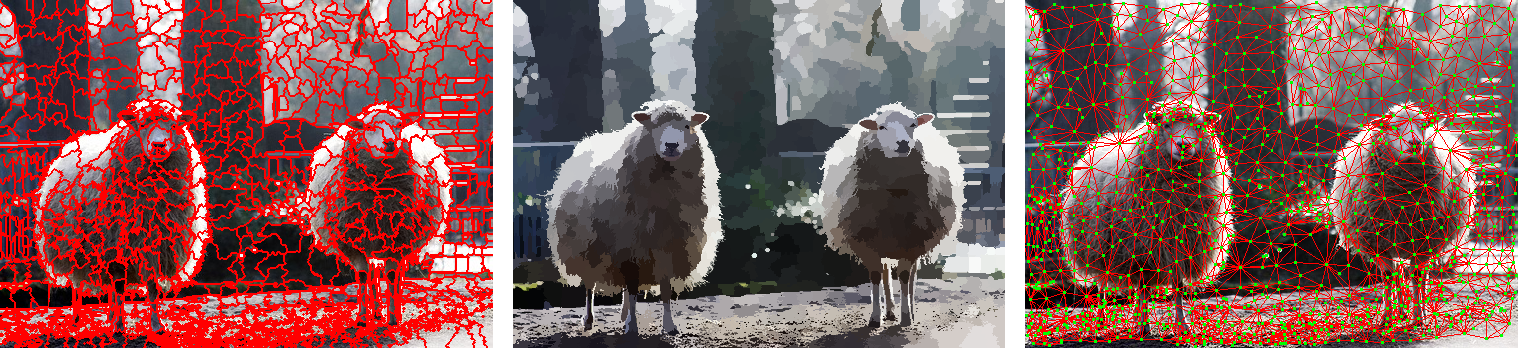
\includegraphics[width=\textwidth]{bilder/pascal_voc_quickshift.png}
}
  \caption[\gls{Pascal}]{Bild aus dem \gls{Pascal} Datensatz, jeweils dargestellt als (1) Originalbild, (2) Superpixelrepräsentation, (3) Durchschnittsfarbe der Superpixel und (4) Graphrepräsentation.}
\label{fig:pascal_voc}
\end{figure}
